%%%%%%%%%%%%%%%%%%%%%%%%%%%%%%%%%%%%%%%%%%%%%%%%%%%%%%%%%%%%%%%%%%%%%%%%%%%%%%%
%Tutorial slides on Python.
%
% Author: FOSSEE
% Copyright (c) 2009, FOSSEE, IIT Bombay
%%%%%%%%%%%%%%%%%%%%%%%%%%%%%%%%%%%%%%%%%%%%%%%%%%%%%%%%%%%%%%%%%%%%%%%%%%%%%%%%

\documentclass[14pt,compress]{beamer}
%\documentclass[draft]{beamer}
%\documentclass[compress,handout]{beamer}
%\usepackage{pgfpages} 
%\pgfpagesuselayout{2 on 1}[a4paper,border shrink=5mm]

% Modified from: generic-ornate-15min-45min.de.tex
\mode<presentation>
{
  \usetheme{Warsaw}
  \useoutertheme{infolines}
  \setbeamercovered{transparent}
}

\usepackage[english]{babel}
\usepackage[latin1]{inputenc}
%\usepackage{times}
\usepackage[T1]{fontenc}

% Taken from Fernando's slides.
\usepackage{ae,aecompl}
\usepackage{mathpazo,courier,euler}
\usepackage[scaled=.95]{helvet}

\definecolor{darkgreen}{rgb}{0,0.5,0}

\usepackage{listings}
\lstset{language=Python,
    basicstyle=\ttfamily\bfseries,
    commentstyle=\color{red}\itshape,
  stringstyle=\color{darkgreen},
  showstringspaces=false,
  keywordstyle=\color{blue}\bfseries}

%%%%%%%%%%%%%%%%%%%%%%%%%%%%%%%%%%%%%%%%%%%%%%%%%%%%%%%%%%%%%%%%%%%%%%
% Macros
\setbeamercolor{emphbar}{bg=blue!20, fg=black}
\newcommand{\emphbar}[1]
{\begin{beamercolorbox}[rounded=true]{emphbar} 
      {#1}
 \end{beamercolorbox}
}
\newcounter{time}
\setcounter{time}{0}
\newcommand{\inctime}[1]{\addtocounter{time}{#1}{\tiny \thetime\ m}}

\newcommand{\typ}[1]{\lstinline{#1}}

\newcommand{\kwrd}[1]{ \texttt{\textbf{\color{blue}{#1}}}  }

%%% This is from Fernando's setup.
% \usepackage{color}
% \definecolor{orange}{cmyk}{0,0.4,0.8,0.2}
% % Use and configure listings package for nicely formatted code
% \usepackage{listings}
% \lstset{
%    language=Python,
%    basicstyle=\small\ttfamily,
%    commentstyle=\ttfamily\color{blue},
%    stringstyle=\ttfamily\color{orange},
%    showstringspaces=false,
%    breaklines=true,
%    postbreak = \space\dots
% }


%%%%%%%%%%%%%%%%%%%%%%%%%%%%%%%%%%%%%%%%%%%%%%%%%%%%%%%%%%%%%%%%%%%%%%
% Title page
\title[Plotting with Python]{Python for Science and Engg: Plotting experimental data}

\author[FOSSEE] {FOSSEE}

\institute[IIT Bombay] {Department of Aerospace Engineering\\IIT Bombay}
\date[] {7 November, 2009\\Day 1, Session 2}
%%%%%%%%%%%%%%%%%%%%%%%%%%%%%%%%%%%%%%%%%%%%%%%%%%%%%%%%%%%%%%%%%%%%%%

%\pgfdeclareimage[height=0.75cm]{iitmlogo}{iitmlogo}
%\logo{\pgfuseimage{iitmlogo}}


%% Delete this, if you do not want the table of contents to pop up at
%% the beginning of each subsection:
\AtBeginSubsection[]
{
  \begin{frame}<beamer>
    \frametitle{Outline}
    \tableofcontents[currentsection,currentsubsection]
  \end{frame}
}

\AtBeginSection[]
{
  \begin{frame}<beamer>
    \frametitle{Outline}
    \tableofcontents[currentsection,currentsubsection]
  \end{frame}
}

% If you wish to uncover everything in a step-wise fashion, uncomment
% the following command: 
%\beamerdefaultoverlayspecification{<+->}

%\includeonlyframes{current,current1,current2,current3,current4,current5,current6}

%%%%%%%%%%%%%%%%%%%%%%%%%%%%%%%%%%%%%%%%%%%%%%%%%%%%%%%%%%%%%%%%%%%%%%
% DOCUMENT STARTS
\begin{document}

\begin{frame}
  \titlepage
\end{frame}

\begin{frame}
  \frametitle{Outline}
  \tableofcontents
  % You might wish to add the option [pausesections]
\end{frame}

\section{Scripts}

\begin{frame}[fragile]
\frametitle{Python Scripts}
  \begin{itemize}
  \item four\_plot.py is called a Python Script
  \item run the file in IPython using \typ{\%run -i four_plot.py}
  \end{itemize}
\end{frame}

\begin{frame}[fragile]
\frametitle{Why would I plot f(x)?}
How often do we plot analytical functions?\\We plot experimental data more.
\begin{small}
\begin{lstlisting}
In []: x = [0, 1, 2, 3]

In []: y = [7, 11, 15, 19]

In []: plot(x, y)
Out[]: [<matplotlib.lines.Line2D object at 0xa73aa8c>]

In []: xlabel('X')
Out[]: <matplotlib.text.Text object at 0x986e9ac>

In []: ylabel('Y')
Out[]: <matplotlib.text.Text object at 0x98746ec>
\end{lstlisting}
\end{small}
\end{frame}

\begin{frame}[fragile]
\begin{figure}
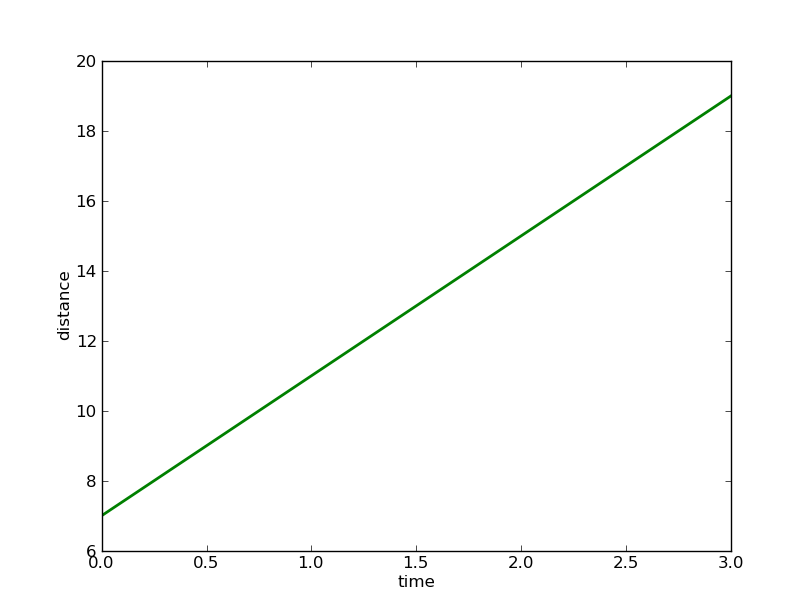
\includegraphics[width=3.5in]{data/straightline.png}
\end{figure}
\alert{Is this what you have?}
\end{frame}

\begin{frame}[fragile]
\frametitle{Plotting points}
\begin{itemize}
\item What if we want to plot the points!
\end{itemize}
\begin{lstlisting}
  In []: clf()

  In []: plot(x, y, 'o')
  Out[]: [<matplotlib.lines.Line2D object at 0xac17e0c>]

  In []: clf()
  In []: plot(x, y, '.')
  Out[]: [<matplotlib.lines.Line2D object at 0xac17e0c>]
\end{lstlisting}
\end{frame}

\begin{frame}[fragile]
\begin{figure}
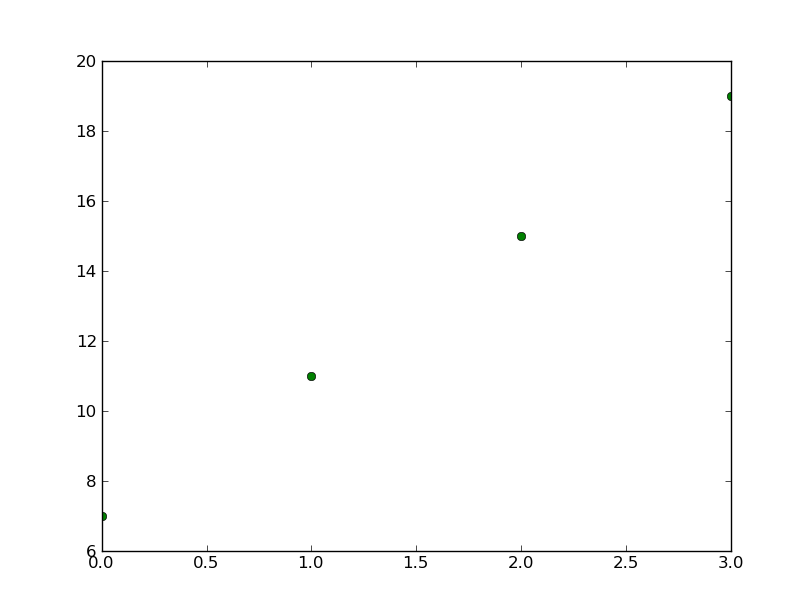
\includegraphics[width=2in]{data/stline_dots.png}
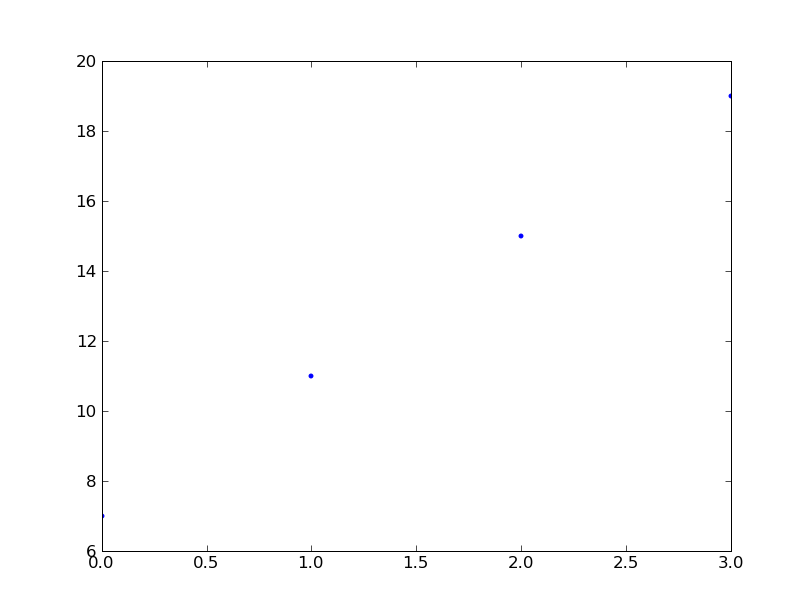
\includegraphics[width=2in]{data/stline_points.png}
\end{figure}
\end{frame}

\begin{frame}[fragile]
\frametitle{Additional Plotting Attributes}
\begin{itemize}
  \item \kwrd{'o'} - Filled circles
  \item \kwrd{'.'} - Small Dots
  \item \kwrd{'-'} - Lines
  \item \kwrd{'- -'} - Dashed lines
\end{itemize}
\end{frame}

\section{Lists}
\begin{frame}[fragile]
  \frametitle{How to create the data?}
What were \typ{x} and \typ{y}?\\
\begin{center}
\alert{\typ{lists!!}}
\end{center}
\begin{lstlisting}
In []: mtlist = [] #Empty List

In []: lst = [ 1, 2, 3, 4, 5] 
\end{lstlisting}
\end{frame}

\begin{frame}[fragile]
\frametitle{Accessing elements of a list}
\begin{lstlisting}
In []: lst[0]+lst[1]+lst[-1]
Out[]: 8
\end{lstlisting}
\end{frame}

\begin{frame}[fragile]
  \frametitle{List: Slicing}
  \begin{block}{Remember\ldots}
	\kwrd{In []: lst = [ 1, 2, 3, 4, 5]}
  \end{block}
\begin{lstlisting}
In []: lst[1:3]  # A slice.
Out[]: [2, 3]

In []: lst[1:-1]
Out[]: [2, 3, 4]
\end{lstlisting}
\alert{\typ{list[initial:final]}}
\end{frame}

%% more on list slicing
\begin{frame}[fragile]
\frametitle{List operations}
\begin{lstlisting}
In []: a = [ 6, 7, 8, 9]
In []: b = lst + a

In []: b
Out[]: [1, 2, 3, 4, 5, 6, 7, 8, 9]

In []: lst.append(6)
In []: lst
Out[]: [ 1, 2, 3, 4, 5, 6]
\end{lstlisting}
%\inctime{10}
\end{frame}

\section{Simple Pendulum}
\begin{frame}[fragile]
\frametitle{Simple Pendulum - L and T}
Let us look at the example of the Simple Pendulum experiment.
\begin{center}
\begin{small}
\begin{tabular}{| c | c | c |}
\hline
$L$ & $T$ & $T^2$ \\ \hline
0.1 & 0.6900 & \\ \hline
0.2 & 0.8989 & \\ \hline
0.3 & 1.1867 & \\ \hline
0.4 & 1.2991 & \\ \hline
0.5 & 1.4656 & \\ \hline
0.6 & 1.5843 & \\ \hline
0.7 & 1.7706 & \\ \hline
0.8 & 1.8296 & \\ \hline
0.9 & 1.9440 & \\ \hline
\end{tabular}
\end{small}\\
\alert{$L \alpha T^2$}
\end{center}
\end{frame}

\begin{frame}[fragile]
\frametitle{Lets use lists}
\begin{lstlisting}
In []: L = [0.1, 0.2, 0.3, 0.4, 0.5, 
            0.6, 0.7, 0.8, 0.9]

In []: T = [0.69, 0.8989, 1.1867, 
            1.2991, 1.4656, 1.5843, 
            1.7706, 1.8296, 1.9440]
\end{lstlisting}
\end{frame}

\begin{frame}[fragile]
\frametitle{Plotting $L$ vs $T^2$}
\begin{itemize}
\item We must square each of the values in T
\item How to do it?
\item We use a \kwrd{for} loop to iterate over T
\end{itemize}
\end{frame}

\begin{frame}[fragile]
\frametitle{Plotting $L$ vs $T^2$}
\begin{lstlisting}
In []: TSq = []

In []: for t in T:
 ....:     TSq.append(t*t)

In []: plot(L, TSq)
Out[]: [<matplotlib.lines.Line2D object at 0xa5b05ac>]
\end{lstlisting}
This gives \kwrd{TSq} which is the list of squares of T values.
\end{frame}

\begin{frame}[fragile]
\begin{figure}
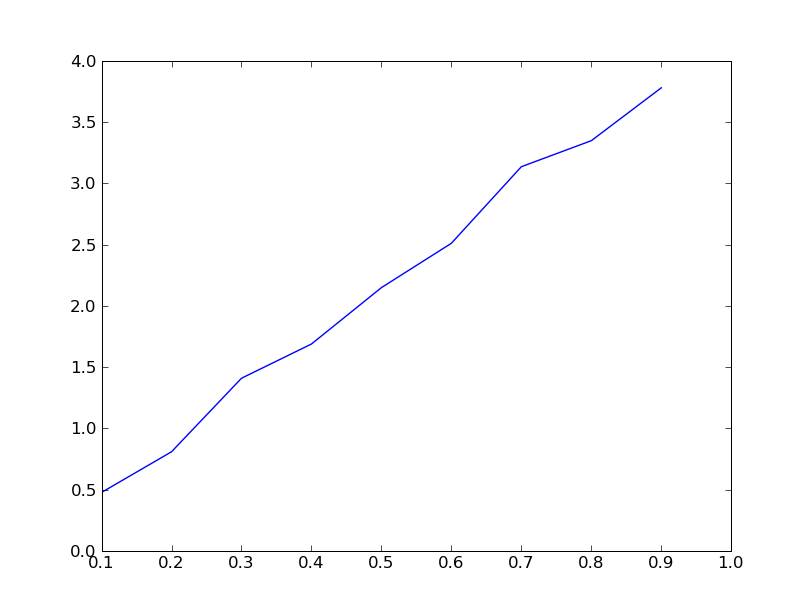
\includegraphics[width=3.5in]{data/L-TSq-limited.png}
\end{figure}
\end{frame}

\begin{frame}[fragile]
\frametitle{What about larger data sets?}
\alert{Data is usually present in a file!} \\
Lets look at the \typ{pendulum.txt} file.
\begin{lstlisting}
$ cat pendulum.txt 
1.0000e-01 6.9004e-01
1.1000e-01 6.9497e-01
1.2000e-01 7.4252e-01
1.3000e-01 7.5360e-01
1.4000e-01 8.3568e-01
1.5000e-01 8.6789e-01
\end{lstlisting}
\ldots
\end{frame}

\begin{frame}[fragile]
\frametitle{Reading \typ{pendulum.txt}}
\begin{itemize}
  \item Let us generate a plot from the data file
  \item File contains L vs. T values 
  \item L - Column1; T - Column2
\end{itemize}
\end{frame}

\begin{frame}[fragile]
\frametitle{Reading \typ{pendulum.txt}}
\begin{lstlisting}
In []: L = []
In []: T = []
In []: for line in open('pendulum.txt'):
  ....     points = line.split()
  ....     L.append(float(points[0]))
  ....     T.append(float(points[1]))
\end{lstlisting}
\begin{itemize}
\item We now have two lists L and T
\item Now, repeat previous steps for plotting
\end{itemize}
\end{frame}

\begin{frame}[fragile]
\frametitle{Plotting from \typ{pendulum.txt}}
\begin{lstlisting}
In []: TSq = []

In []: for t in T:
 ....:     TSq.append(t*t)

In []: plot(L, TSq, '.')
\end{lstlisting}
\end{frame}

\begin{frame}[fragile]
\begin{figure}
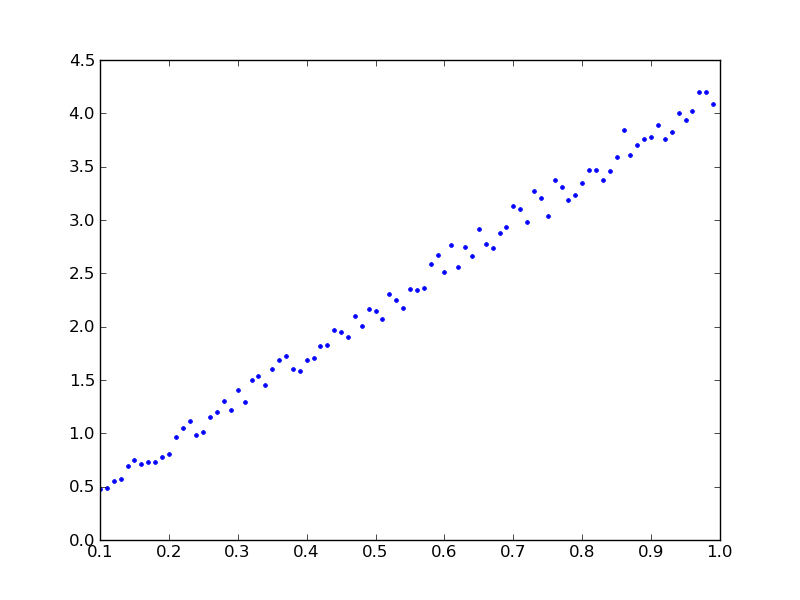
\includegraphics[width=3.5in]{data/L-Tsq.png}
\end{figure}
\end{frame}

\begin{frame}[fragile]
  \frametitle{Reading files \ldots}
\typ{In []: for line in open('pendulum.txt'):}
\begin{itemize}
\item opening file `\typ{pendulum.txt}'
\item reading the file line by line
\item \typ{line} is a \kwrd{string}
\end{itemize}
\end{frame}

\section{Strings}
\begin{frame}[fragile]
\frametitle{Strings}
Anything within ``quotes'' is a string!
\begin{lstlisting}
' This is a string '  
" This too! "
""" This one too! """
''' And one more! '''
\end{lstlisting}
\end{frame}

\begin{frame}[fragile]
\frametitle{Strings and \typ{split()}}
  \begin{lstlisting}
In []: greet = 'hello world'

In []: greet.split()
Out[]: ['hello', 'world']
  \end{lstlisting}
This is what happens with \typ{line}
  \begin{lstlisting}
In []: line = '1.2000e-01 7.4252e-01'

In []: line.split()
Out[]: ['1.2000e-01', '7.4252e-01']
  \end{lstlisting}
\end{frame}

\begin{frame}[fragile]
\frametitle{Getting floats from strings}
  \begin{lstlisting}
In []: type(points[0])
Out[]: <type 'str'>
  \end{lstlisting}
But, we need floating point numbers
  \begin{lstlisting}
In []: t = float(points[0])

In []: type(t)
Out[]: <type 'float'>
  \end{lstlisting}
\end{frame}

\begin{frame}[fragile]
\frametitle{Let's review the code}
\begin{small}
\begin{lstlisting}
In []: L = []
In []: T = []
In []: for line in open('pendulum.txt'):
  ....     points = line.split()
  ....     L.append(float(points[0]))
  ....     T.append(float(points[1]))

In []: TSq = []

In []: for t in T:
 ....:     TSq.append(t*t)

In []: plot(L, TSq, '.')
\end{lstlisting}
\end{small}
\end{frame}

\begin{frame}[fragile]
\begin{figure}
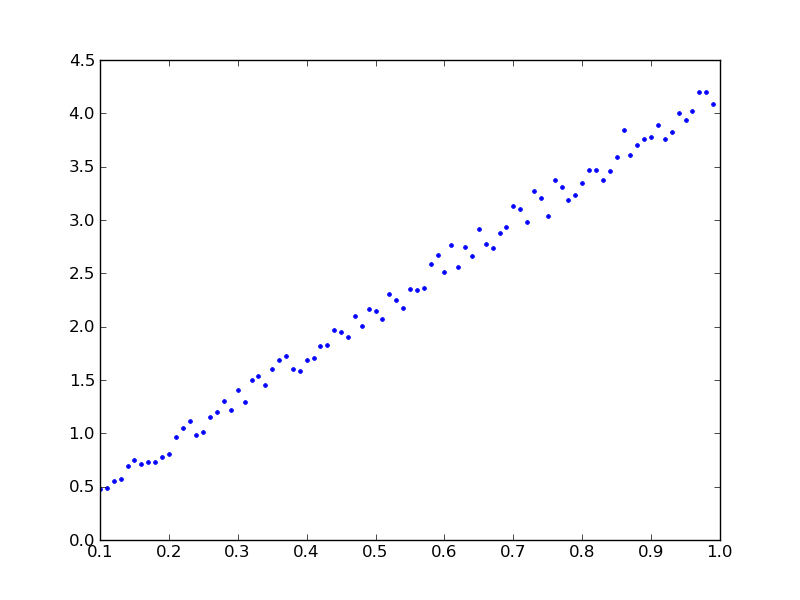
\includegraphics[width=3.5in]{data/L-Tsq.png}
\end{figure}
\end{frame}

\section {Summary}
\begin{frame}[fragile]
\frametitle{What did we learn?}
\begin{itemize}
  \item Python scripts
  \item \kwrd{\%run -i}
  \item Plotting points
  \item Plot attributes
  \item Lists
  \item \kwrd{for}
  \item Reading files
  \item Strings
\end{itemize}
\end{frame}

\end{document}
